\documentclass[sigconf,nonacm]{acmart}
\usepackage{booktabs}
\usepackage{fancyvrb}
\usepackage{wrapfig}
\usepackage{listings}
% dcg grammar panels: nonterminals blue, leaves red (matching the
% grid figure's two tree colors), "% e.g." snippets grey italic
\lstdefinestyle{dcg}{
  basicstyle=\ttfamily\scriptsize,
  commentstyle=\color{gray}\itshape,
  comment=[l]{\%},
  alsoletter={_},
  keywordstyle=\color{blue!70!black}\bfseries,
  morekeywords={intro,hook,gap,elevator,move,rqs,contribs,lit,
    scheme,wings,ours,holes,issues,pivot,methods,data,rig,
    baselines,measures,stats,hyperparams,ttv,paper,litreview,
    results,result,discussion,observations,threats},
  keywordstyle=[2]\color{red!65!black},
  morekeywords=[2]{quantified_pain,anchor,setting,problem,
    naive_fails,prior_fails,key_idea,epigram,this_paper_does,
    christening,rq,answer,contrib,repro_url,caveat,roadmap,
    axes,wing,where_we_sit,crowded,empty,issue,claimed,deferred,
    source,filters,step,rival,metric,tests,thresholds,settings,
    justification,ablation,worked_example,construct,internal,
    external,conclusion,charts,comments,observation,summary,
    future_work},
  frame=single,
  keepspaces=true}
% python tutorial listings (appendix stats): inconsolata is
% already acmart's tt face; just add color + light frame
\lstdefinestyle{py}{
  language=Python,
  basicstyle=\fontsize{8}{8.7}\selectfont\ttfamily,
  keywordstyle=\color{blue!70!black}\bfseries,
  stringstyle=\color{red!65!black},
  commentstyle=\color{gray}\itshape,
  emph={len,sorted,min,max,abs,mean,stdev,lambda},
  emphstyle=\color{teal!60!black},
  escapechar=|,
  showstringspaces=false,
  columns=flexible,
  keepspaces=true,
  xleftmargin=1em,
  frame=leftline,
  framerule=0.8pt,
  rulecolor=\color{black!30},
  aboveskip=0.8em, belowskip=0.8em}
\usepackage{array}
\usepackage{colortbl}
\usepackage{tikz}
\usetikzlibrary{decorations.pathmorphing}
\settopmatter{printfolios=true}
% generated by litfig.py; do not hand-edit
\newcommand{\litFetched}{249}
\newcommand{\litSE}{249}
\newcommand{\litKnee}{23}
\newcommand{\litRead}{26}
\newcommand{\litKneeCites}{31}
\newcommand{\litWingA}{1,000}
\newcommand{\litWingB}{788}
\newcommand{\litBoth}{285}
\newcommand{\litAbs}{26}
\newcommand{\litTPH}{2}
\newcommand{\litNone}{2}
\newcommand{\litRefs}{2,239}
\newcommand{\litClassics}{73}
\newcommand{\litCiting}{1,882}
\newcommand{\litOwn}{3}


% review comments: \note{who}{what}; resolve = delete.
% make notes lists them all. acmart already loads xcolor.
\newcommand{\note}[2]{\textcolor{red}{\textbf{[#1: #2]}}}

% pause-and-review call-out boxes: \begin{pause}{topic}...
\newcounter{pausebox}
\newsavebox{\pauseboxsave}
\newenvironment{pause}[1]{%
  \refstepcounter{pausebox}\par\medskip\noindent
  \begin{lrbox}{\pauseboxsave}%
  \begin{minipage}{\dimexpr\linewidth-9mm}%
  \small\noindent
  \textbf{\textsc{Pause \& review \thepausebox: #1}}\\[0.2em]}%
 {\end{minipage}\end{lrbox}%
  \noindent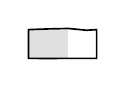
\begin{tikzpicture}
  \node[inner sep=5pt, anchor=west] (b) at (5mm,0)
    {\usebox{\pauseboxsave}};
  \fill[black!12]
    ([xshift=-5mm]b.north west) rectangle (b.south west);
  \draw[decorate, decoration={random steps, segment length=7pt,
    amplitude=0.7pt}, line width=0.6pt]
    ([xshift=-5mm]b.north west) -- (b.north east) --
    (b.south east) -- (b.south west) --
    ([xshift=-5mm]b.south west) -- cycle;
  \end{tikzpicture}\par\medskip}

% compact author block: one names line, one affils line
\makeatletter
\renewcommand\@authorfont{\Large\sffamily}
\renewcommand\@affiliationfont{\normalsize}
\makeatother

\title{Follow Your Strengths: Writing Papers with LLMs}
% \note in title breaks headers; working title, timm to confirm.

\author{Tim Menzies\textsuperscript{1},
  Carmen Armenti\textsuperscript{2},
  Dario Di Nucci\textsuperscript{3},\\
  Matteo Esposito\textsuperscript{4},
  Valentina Lenarduzzi\textsuperscript{4},
  Klaus Schmid\textsuperscript{5}}
\affiliation{\institution{%
  \textsuperscript{1}NC State, USA;
  \textsuperscript{2}USI, Switzerland;
  \textsuperscript{3}Univ.~Salerno, Italy;\\
  \textsuperscript{4}Univ.~Southern Denmark;
  \textsuperscript{5}Univ.~Hildesheim, Germany\\
  timm@ieee.org; carmen.armenti@usi.ch; d.dinucci@ieee.org;\\
  \{esposito,lenarduzzi\}@imada.sdu.dk; schmid@sse.uni-hildesheim.de}\country{}}

\begin{abstract}
Paper writing consumes time that should go to research; newcomers lack
a teachable method; large language models offer speed but generate
bland prose.
This paper offers a method guided by Newell's advice (know your own
strengths and follow them) and by an experience base that LLMs can
mine from the research corpus in minutes.
The method decomposes writing into small checkable steps, matches a
researcher's demonstrated strengths to a field's open problems, and
critiques its own drafts.
\note{claude}{one results sentence once paper0 has results}
\end{abstract}


\keywords{LLM agents, research writing, strengths, experience base,
  science of science}

\begin{document}
\maketitle

\section{Introduction}

Three problems motivate this paper.
Firstly, newcomers need guidance in the craft of writing research
papers, and the standard advice is scattered across decades of
folklore.
Secondly, established researchers struggle to find time for research,
since writing papers (and maturing the papers of graduate students)
has grown into a full-time job.
This burden is measurably heavy in software engineering: by one
estimate, one SE paper costs over four times the collaborative effort
of one machine learning paper (4.09 versus 0.86 ICLR
points~\cite{luo25,menzies26se}).
Thirdly, when authors turn to large language models for help, those
models generate prose that is bland, verbose, and instantly
recognizable as machine written.

Our response takes guidance from two sources.
The first is Newell's advice to a young scientist: know your own
strengths and follow them~\cite{newell91}.
\note{timm}{Mary Shaw retells this advice; need the exact talk or
essay to cite for the Shaw connection.}
Applied to paper writing, that advice yields a workflow of small
interim steps, and it gives teams a natural division of labor (what
unique strengths does each member bring?).
Hence it addresses our first problem, since a workflow of explicit
steps is teachable in a way that folklore is not.

The second source is an experience base; that is, a database, reverse
engineered from the SE corpus, of state-of-the-art results, holes in
that state of the art, and the experimental standards of particular
sub-fields.
Using LLMs, hundreds of papers can be downloaded and parsed for this
material in minutes.
Hence our second problem shrinks, since months of manual reading
becomes a background job.
Further, \textbf{it is now possible to reverse engineer, from a
researcher's own papers, what their particular strengths are and how
those strengths might attack current problems in the field}.
To our knowledge, that inversion was impractical before LLMs.

Three services augment these two ideas: (a) a catalog of anti-patterns
seen in LLM-generated text, with rules for avoiding them; (b) a map of
the common structures of research papers; and (c) automatically
generated critiques which, acting as ICSE's reviewer two, report the
weaknesses of the current draft and propose a revision that avoids at
least some of them.
Hence our third problem also yields, since LLM prose need not be bland
once the machine is told, precisely, what bland looks like.

Before starting, one frequently asked question deserves an answer.
Should we follow Newell's advice at all?
If everyone focuses on their own tricks, each of us risks the guilt of
the hammer that sees only nails.
Our short reply is that strengths choose the tools while the field's
open problems choose the targets; hence the hammer is aimed, not
wandering.
A longer reply appears in the companion paper.
\note{timm}{cite paper1 here once it has a public handle}
\note{claude}{roadmap paragraph goes here once paper0's sections
exist}

\section{Know Thyself}

\begin{quote}
{\em Know thyself.} --- inscribed on the Temple of Apollo at Delphi
\end{quote}

Newell's advice cannot be followed until the strengths are named, and
self-report names them badly.
Hence, before diving deep into any literature, we first reverse
engineer the team from the record of its own papers.

Our instrument is the repertory grid of Kelly's personal construct
theory~\cite{kelly55}.
Kelly held that people make sense of a domain through bipolar
distinctions ({\em constructs}) of their own devising.
A grid is elicited by triads: pick three team members, ask which one
stands apart from the other two and on what dimension; each answer
yields one construct; repeat until no new dimensions appear; then rate
everyone on every construct.

Data collection took minutes.
For six of this paper's authors, an LLM agent fetched each author's
five most-cited papers of all time and of the last five years
(scanning some 1,200 paper records), coded them against the ICSE'27
research-track areas, then played triad interviewee.
Constructs agreeing above 90\% were merged.
Figure~\ref{fig:focus} shows the result after FOCUS sorting: rows and
columns reordered so similar neighbors adjoin, poles reversed to
align, and trees built by merging adjacent clusters
only.\footnote{Caveats: one rater (the agent), citation counts as the
sole proxy for strength, and two early-career authors rated on very
few papers.}

\begin{figure}[t]
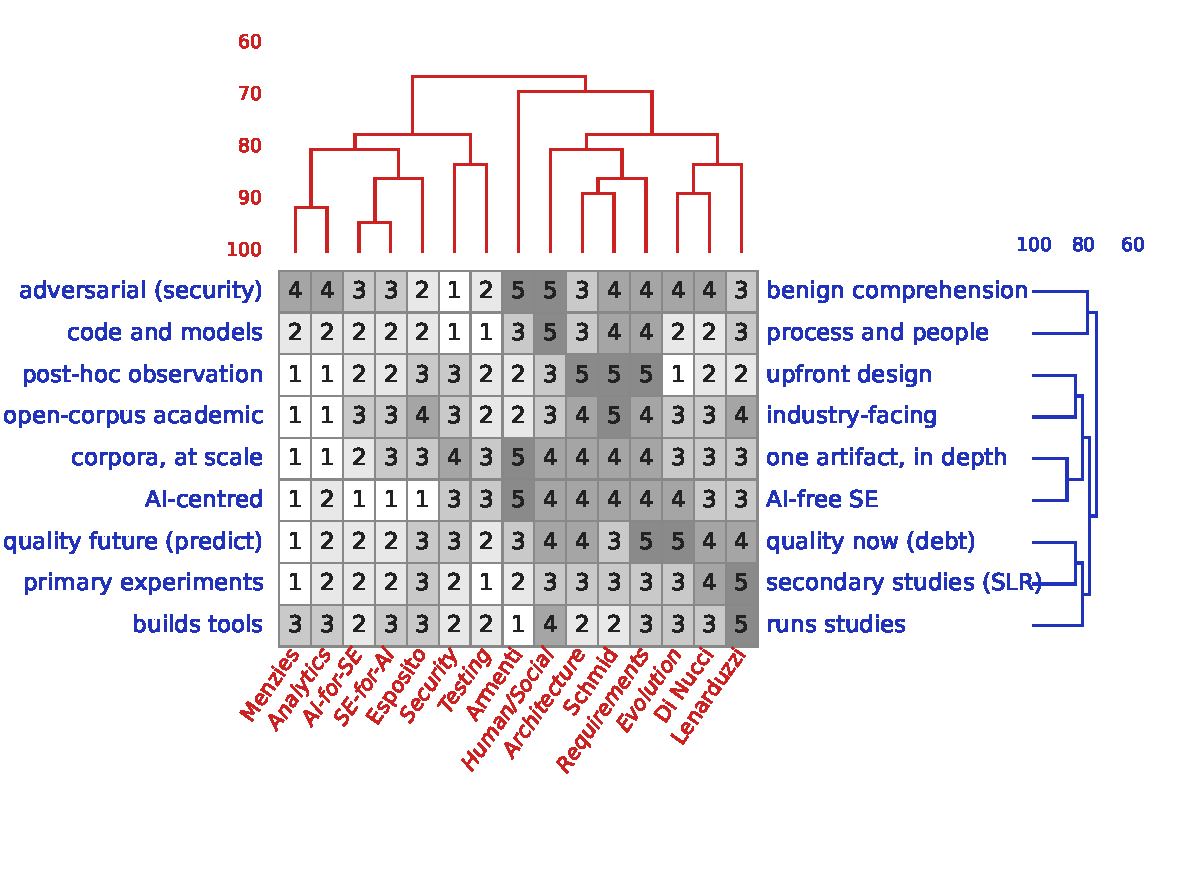
\includegraphics[width=\linewidth]{fig/focus_grid}
\caption{Repertory grid of six authors (upright columns)
plus the nine ICSE'27 areas as reference elements (italic columns; see
\S\ref{sec:map}).
Grey cells score each column from the left pole (1) to the right pole
(5) of each construct; trees join neighbors by percentage match;
regenerate via {\em make focus}.}
\label{fig:focus}
\end{figure}

The grid rewards three readings.
Firstly, near-synonyms: construct rows that merge early name one local
dimension twice.
In this team, working at corpus scale co-travels with being
AI-centred, as does primary experimentation with future-facing
prediction.
Secondly, birds of a feather: Lenarduzzi and Di Nucci match at around
90\%, a tight quality-and-evolution core that anchors the team.
Thirdly, complements: Schmid and Armenti lie farthest from that core,
so upfront design and single-artifact comprehension are scarce skills
here, present in exactly one member each.
Hence the grid is at once a division of labor and a price list of the
team's blind spots, computed before reading a single outside paper.

\section{Mapping the Team to the Field}
\label{sec:map}

Newell's third and fourth questions ask where a team could work and
what important issues live there.
For a working list of "where", we borrow the nine areas of the ICSE'27
research track: AI for SE; analytics; architecture and design;
dependability and security; evolution; human and social aspects;
requirements and modeling; SE for AI; and testing and analysis.

Rather than tabulate those areas separately, we score each area on the
same nine constructs as the people and add them to
Figure~\ref{fig:focus} as reference elements (the italic columns).
Each such column is an archetype: how the typical highly cited
researcher of that area would rate, judged from the track descriptions
rather than measured from a corpus.
\note{claude}{upgrade path: build each area column from its ICSE
distinguished papers of the last five years, coded like the author
papers; then people and areas share one provenance} The red tree then
answers a question a topic list cannot: who stands nearest which area.
Some pairings are strong: Menzies sits at 92\% match to analytics, Di
Nucci at 89\% to evolution, Schmid at 89\% to both requirements and
architecture, Esposito at 86\% to SE for AI.
Others are loose: Lenarduzzi's nearest areas (evolution, architecture)
reach only 72\%, and Armenti's (human and social aspects) 69\%, so
those two are less typecast than the rest of us.
Hence question three answers itself: the team's natural territories
are the areas already adjacent to one of its members.

The far columns matter as much as the near ones.
No author sits within 85\% of security (best: Esposito, 78\%) or
testing (best: 72\%); those two areas cling to each other, not to a
person.
That is the priced blind spot of this team: papers there would be
written against the grain, or with a new collaborator who brings that
column closer.

\section{Reading In}
\label{sec:lit}

A topic chosen is a literature owed.
Our lit-review rules are few enough to fit in a box:
Figure~\ref{fig:prompt} shows the whole prompt, whose first three
lines are machine-read configuration and whose rules drive the
pipeline.

\begin{figure}[t]
\fbox{\parbox{\dimexpr\linewidth-2\fboxsep-2\fboxrule}{\small
{\ttfamily goal:~~human factors of AI assistants\\ \hspace*{4.2em}for
[software engineering]\\ years:~2021-2026\\ seed:~~(one anchor DOI per
wing)}\\[0.4em] Rules: (1)~define ``recent'' by field velocity: ten
years default, two to three for LLM-speed fields; (2)~the bracketed
goal term is a venue filter: the initial grab searches only inside
that field's venues, per a reviewable venue list;\footnote{Sources for
the list: se-deadlines.github.io, Google Scholar's venue index for
``software engineering'', OpenAlex sources whose names contain
``software'', and the venues of the team's own recent papers.
CORE no longer lists journals.}
(3)~sort the hits by citations and read above the knee of that curve
(the point farthest from the first-to-last chord); (4)~seeds join the
reading set regardless of the knee; (5)~snowballing is unrestricted:
backward from the reading set for the classics and forward from the
seeds for the newest work, roaming outside the field on purpose;
(6)~the download rate is a finding: report it, never silently drop
missing papers.
Then code every abstract; hunt for subsets and their overlaps; and
list which of the team's own papers already sit inside the set.}}
\caption{The prompt that runs the literature review
(from the rite engine's search rules, github.com/timm/rite).}
\label{fig:prompt}
\end{figure}

\begin{figure}[t]
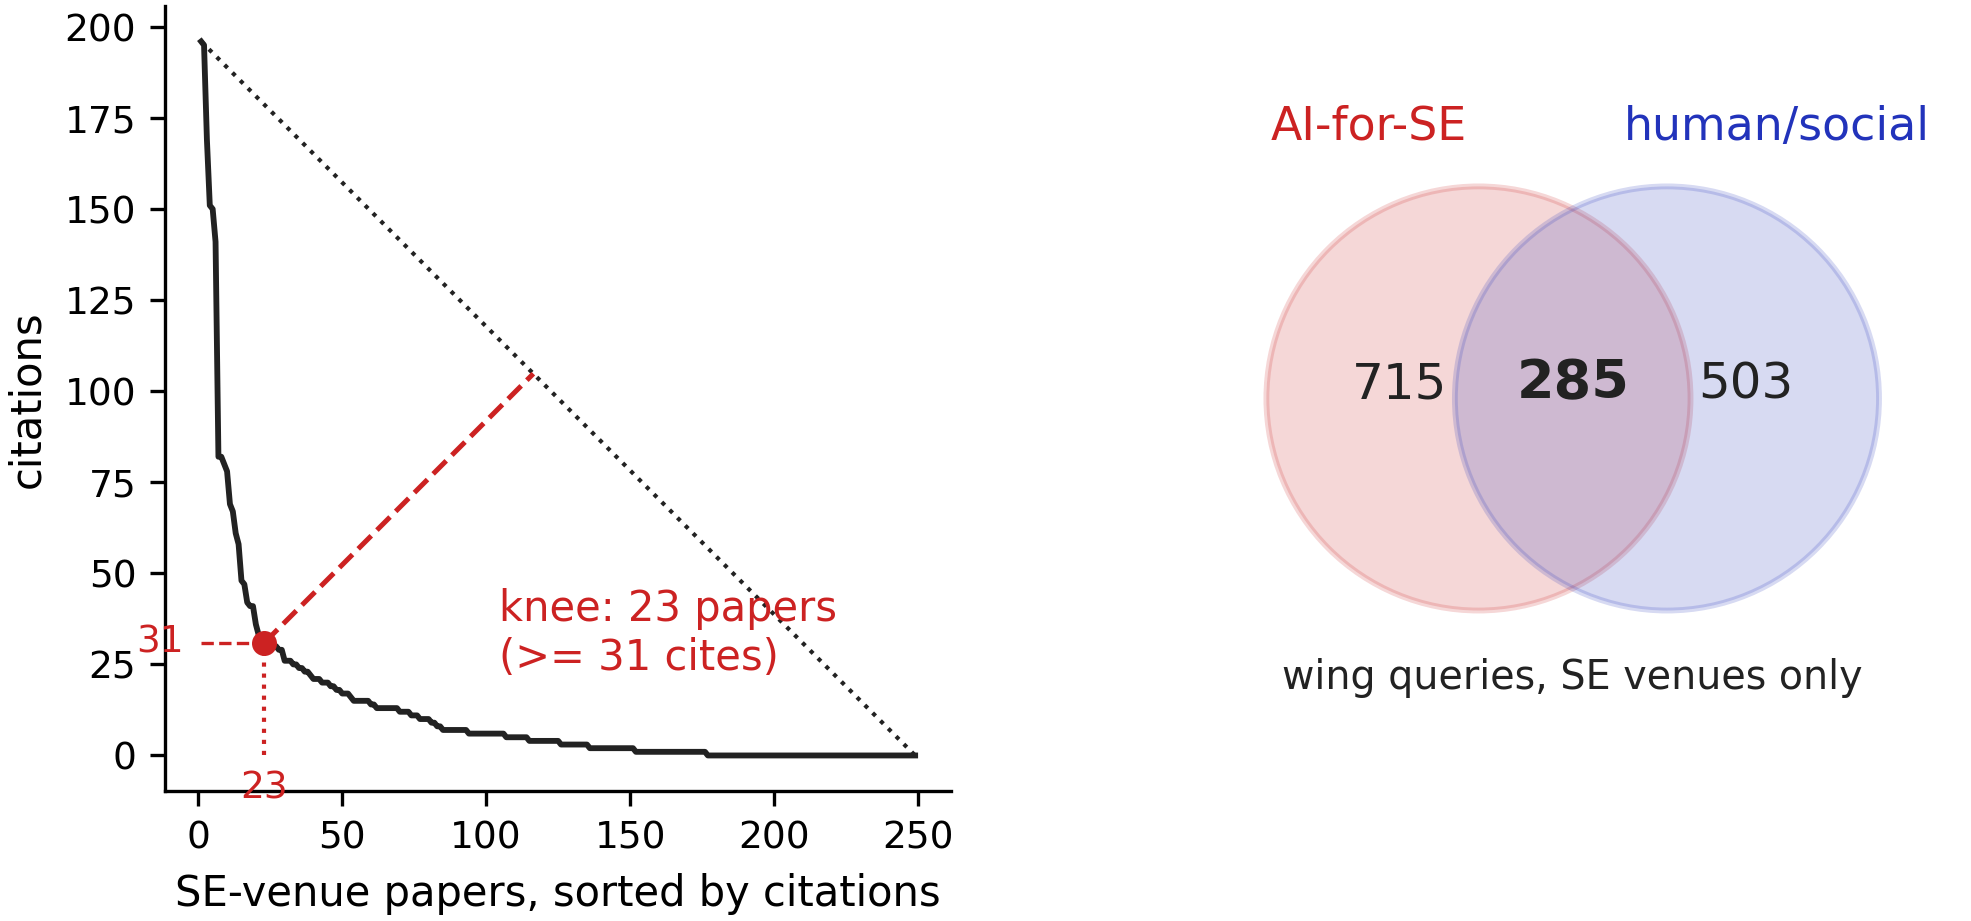
\includegraphics[width=\linewidth]{fig/lit}
\caption{Left: the sorted-cites curve of the goal
query, searched within SE venues only (\litSE{} papers, OpenAlex,
2021--2026).
The dotted line joins the most- to the least-cited paper; the dashed
drop marks the point farthest from that line, i.e.\ the knee:
\litKnee{} papers at \litKneeCites{} citations or more.
Right: the two wings as separate queries, same venues; their
\litBoth-paper overlap.
Regenerate via {\em litfig.py}.}
\label{fig:lit}
\end{figure}

Figure~\ref{fig:lit} shows the rules running on the area that
\S\ref{sec:map} chose.
The venue rule earned its place twice.
A first draft of this section skipped it, and the reading set filled
with general AI blockbusters (a machine learning survey, the GPT-4
report, a metaverse position paper) from venues nowhere near software
engineering.
A second draft filtered venues after a citation-sorted fetch, and that
failed too: of the top 1{,}000 hits, only nine sat in SE venues, since
mega-cited outsiders crowd out the field long before the filter runs.
Hence the venue list joins the query itself, and the human hours are
spent only on papers our field would recognize.

\begin{figure}[t]
\centering
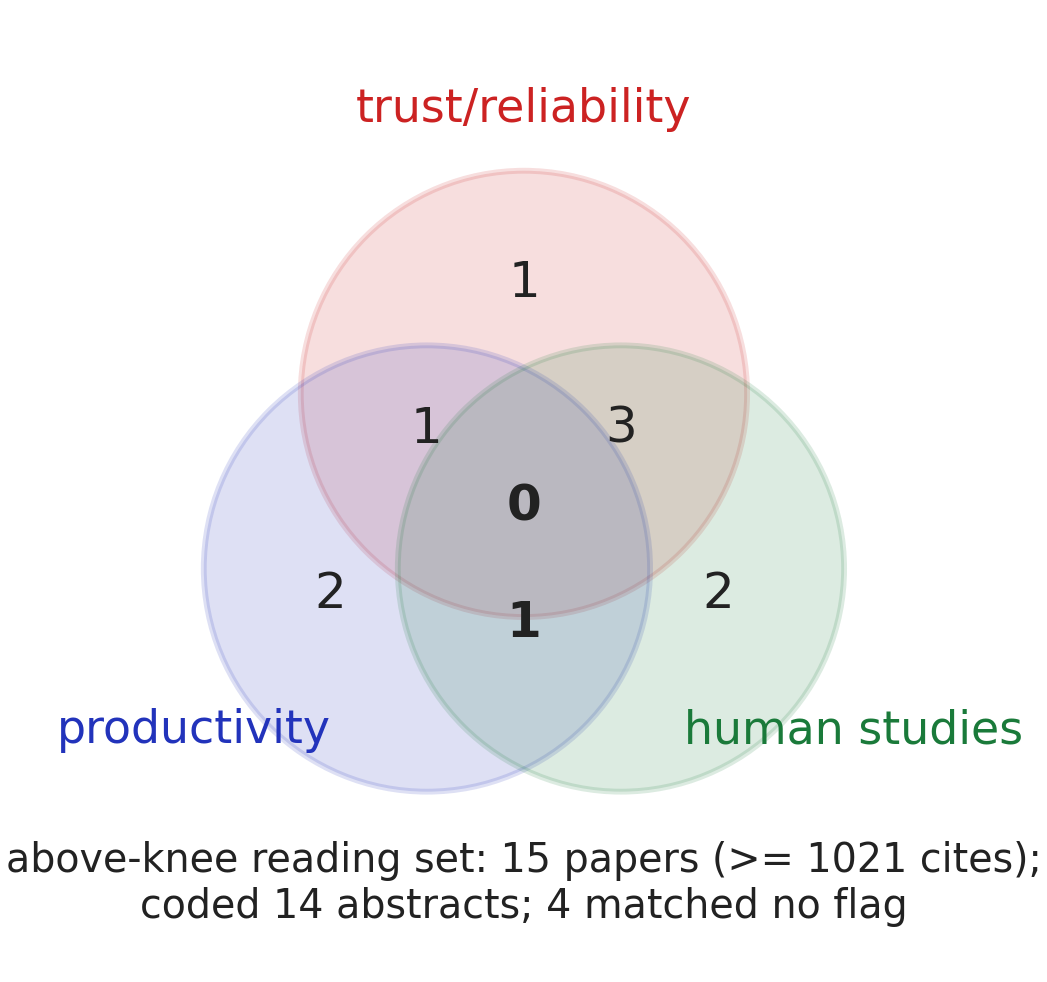
\includegraphics[width=0.62\linewidth]{fig/lit2}
\caption{The reading set (\litRead{} papers: the
\litKnee{} above the knee of Figure~\ref{fig:lit}, plus three seeds),
coded against three topic flags.
Regenerate via {\em litfig.py}.}
\label{fig:lit2}
\end{figure}

The reading set is what sits above the knee, plus the seeds that
rule~(4) admits regardless of citations: \litRead{} papers in all, of
which \litAbs{} had retrievable abstracts.
Here the seeds are the team's own three in-query papers (rows marked
``s'' in Table~\ref{tab:read}).
Figure~\ref{fig:lit2} codes those with three topic flags (trust,
productivity, human-method); \litTPH{} papers occupy all three
circles, and \litNone{} match no flag.
Table~\ref{tab:read} lists the reading set itself, with its flags.

\begin{table*}[t]
\caption{The reading set: title (first author), venue,
year, citations, and the three topic flags of Figure~\ref{fig:lit2}.
Rows marked ``s'' are seeds: the team's own in-query papers,
admitted regardless of the knee.
Generated by {\em litfig.py} from OpenAlex; venues as recorded there.}
\label{tab:read}
\scriptsize \setlength{\tabcolsep}{3pt}
\centering
% generated by litfig.py; do not hand-edit
\begin{tabular}{@{}rp{0.58\linewidth}p{0.17\linewidth}rr@{}}
\toprule
\# & paper & venue & year & cites\\
\midrule
1 & Machine Learning: Algorithms, Real-World Application... (Sarker) & SN Computer Science & 2021 & 5221\\
2 & Opinion Paper: “So what if ChatGPT wrote it?” Multid... (Dwivedi) & International Journal  & 2023 & 3869\\
3 & Metaverse beyond the hype: Multidisciplinary perspec... (Dwivedi) & International Journal  & 2022 & 2619\\
4 & Machine learning and deep learning (Janiesch) & Electronic Markets & 2021 & 2534\\
5 & GPT-4 Technical Report (OpenAI) & arXiv (Cornell Univers & 2023 & 2421\\
6 & A Metaverse: Taxonomy, Components, Applications, and... (Park) & IEEE Access & 2022 & 1789\\
7 & Natural language processing: state of the art, curre... (Khurana) & Multimedia Tools and A & 2022 & 1762\\
8 & ARTIFICIAL INTELLIGENCE FOR THE REAL WORLD (?) & International Research & 2023 & 1450\\
9 & A survey on large language model based autonomous ag... (Wang) & Frontiers of Computer  & 2024 & 1284\\
10 & Flamingo: a Visual Language Model for Few-Shot Learn... (Jean-Baptiste) & arXiv (Cornell Univers & 2022 & 1247\\
11 & Generative AI (Feuerriegel) & Business \& Informatio & 2023 & 1241\\
12 & A SWOT analysis of ChatGPT: Implications for educati... (Farrokhnia) & Innovations in Educati & 2023 & 1212\\
13 & A Review of Artificial Intelligence (AI) in Educatio... (Zhai) & Complexity & 2021 & 1168\\
14 & AI-Based Modeling: Techniques, Applications and Rese... (Sarker) & SN Computer Science & 2022 & 1114\\
15 & Hydrogen production, storage, utilisation and enviro... (Osman) & Environmental Chemistr & 2021 & 999\\
16 & Deep learning modelling techniques: current progress... (Ahmed) & Artificial Intelligenc & 2023 & 997\\
17 & The future landscape of large language models in med... (Clusmann) & Communications Medicin & 2023 & 981\\
18 & Unmanned aerial vehicles (UAVs): practical aspects, ... (Mohsan) & Intelligent Service Ro & 2023 & 967\\
19 & A Survey on the Explainability of Supervised Machine... (Burkart) & Journal of Artificial  & 2021 & 966\\
20 & New Era of Artificial Intelligence in Education: Tow... (Kamalov) & Sustainability & 2023 & 956\\
21 & Artificial intelligence and smart vision for buildin... (Baduge) & Automation in Construc & 2022 & 935\\
22 & Using machine learning approaches for multi-omics da... (Reel) & Biotechnology Advances & 2021 & 900\\
23 & A Review of the Role of Artificial Intelligence in H... (Kuwaiti) & Journal of Personalize & 2023 & 838\\
24 & Unlocking the value of artificial intelligence in hu... (Chowdhury) & Human Resource Managem & 2022 & 829\\
25 & A survey on deep learning tools dealing with data sc... (Alzubaidi) & Journal Of Big Data & 2023 & 823\\
26 & Smart wearable devices in cardiovascular care: where... (Bayoumy) & Nature Reviews Cardiol & 2021 & 819\\
27 & Adaptive Learning Using Artificial Intelligence in e... (Gligorea) & Education Sciences & 2023 & 819\\
28 & <scp>ChatGPT</scp> and a new academic reality: <scp>... (Lund) & Journal of the Associa & 2023 & 790\\
29 & Human resource management in the age of generative a... (Budhwar) & Human Resource Managem & 2023 & 790\\
30 & Challenges and Opportunities of Generative AI for Hi... (Michel‐Villarreal) & Education Sciences & 2023 & 780\\
31 & Survey on 6G Frontiers: Trends, Applications, Requir... (Alwis) & IEEE Open Journal of t & 2021 & 776\\
32 & A Review on Large Language Models: Architectures, Ap... (Raiaan) & IEEE Access & 2024 & 738\\
33 & AI Tools in Society: Impacts on Cognitive Offloading... (Gerlich) & Societies & 2025 & 732\\
34 & Academic Integrity considerations of AI Large Langua... (Perkins) & Journal of University  & 2023 & 706\\
35 & ChatGPT and Open-AI Models: A Preliminary Review (Roumeliotis) & Future Internet & 2023 & 697\\
36 & Retrieval-Augmented Generation for Large Language Mo... (Gao) & arXiv (Cornell Univers & 2023 & 686\\
37 & The impact of big data analytics and artificial inte... (Benzidia) & Technological Forecast & 2021 & 675\\
38 & Teachers’ AI digital competencies and twenty-first c... (Ng) & Educational Technology & 2023 & 612\\
\bottomrule
\end{tabular}

\end{table*}

Snowballing then ran from that set, deliberately unfiltered by venue,
since good ancestors and good critics live anywhere: backward
collection found \litRefs{} distinct references (\litClassics{} cited
by two or more of the reading set: the candidate classics); forward
collection found \litCiting{} works already citing the reading set.
\note{timm}{the three flags are paper0-local; a full run would fork
its own workdir and flags.py, per the engine rules}

The process itself yielded findings worth recording.
Full texts are scarce: in this workdir's companion pipeline run, only
22 of 54 chased PDFs (41\%) could be downloaded; abstracts come easier
(here, \litAbs{} of \litKnee).
Google Scholar is closed to scripts; OpenAlex, Semantic Scholar, and
arXiv answer machine queries gladly, so the pipeline builds only on
the willing.
An earlier full-text pass showed abstract-only coding missing about
half the flags; hence full text is coded above the knee.
Finally, the own-papers rule paid off: \litOwn{} papers by this team
(Di Nucci on accessibility, Schmid on MLOps, Esposito on AI agents)
already sit in the venue-filtered goal results.
The territory is adjacent to us without yet being occupied by us.

Reading done, the loop starts writing.
Figure~\ref{fig:sample} shows what that looks like: the step-8 draft
(title, elevator speech, abstract, questions, contributions) plus the
step-9 lit-review pivot, generated for the very topic that
\S\ref{sec:map} nominated, then frozen here as an exhibit rather than
polished into a claim.

\begin{figure*}[b!]
\fbox{\begin{minipage}{\dimexpr\textwidth-2\fboxsep-2\fboxrule}
\small
\begin{center}
{\scshape\bfseries Example output (synthetic)}\\[0.1em]
{\footnotesize What the loop emits at step 8 for the topic
nominated in \S\ref{sec:map}; unedited machine draft, before the
critics of steps 10--14. Nothing here is a measured claim of this
paper.}
\end{center}
\vspace{0.3em}
\begin{minipage}[t]{0.47\textwidth}
\textbf{paper[0]: title, elevator speech, abstract.}\\[0.3em]
{\em Do AI Assistants Amplify or Erase a Team's Measured
Strengths?}\\[0.4em]
\begin{quote}
Six researchers, measured from their own corpus, split into a wing
that measures and a wing that crafts.
When LLM assistants join the loop, does the work drift toward those
peaks, or toward the model's mean?
We propose an instrument that answers this per team, in minutes,
from public records.
\end{quote}
{\em Abstract:} Teams adopt LLM writing assistants faster than they
can measure the effect on their own output.
We reverse engineer a team's strengths from its published corpus
(repertory grid over coded papers, FOCUS sorted), instrument one
year of assisted and unassisted writing, and measure drift between
the two against the team's own baseline.
The instrument runs from public records in minutes.
Scripts, data, and grids: github.com/timm/how2rite.
\end{minipage}\hfill
\begin{minipage}[t]{0.47\textwidth}
\textbf{Research questions} (answers land inline, in bold, once
step 9's experiments run).\\
RQ1: Can a team's strengths be recovered from its public corpus
alone?\\
RQ2: Does assisted output sit nearer the team's measured centroid,
or the model's default register?\\
RQ3: Which member-to-area pairings does the drift evidence
support?\\[0.5em]
\textbf{Contributions.}
(1)~a corpus-derived strengths instrument (grid plus FOCUS sort);
(2)~a measured map of six researchers against the nine ICSE'27
areas;
(3)~blend arithmetic that nominates cross-wing topics;
(4)~a replication package: github.com/timm/how2rite.\\[0.5em]
\textbf{Step 9, the lit-review pivot} (form: respect, then
disrespect, then the open-issues list).\\[0.3em]
Prior work earns respect on two fronts: trust in AI assistants is
now measured at the level of the individual developer, and
productivity effects are quantified across thousands of sessions.
However, the corpora end where teams begin: the trust studies
observe single subjects, and the productivity numbers average away
exactly the between-member differences that define a team.
Based on the above, three issues remain open: (i)~team-level
measures of strength, (ii)~drift of assisted output against such
measures, and (iii)~longitudinal designs that separate tool effects
from team learning.
The sections that follow address (i) and (ii); issue (iii) is
future work.
\end{minipage}
\end{minipage}}
\caption{A worked sample of the loop's own prose products, boxed
and labeled so no reader mistakes it for a result.
The form follows the engine's structure rules (github.com/timm/rite):
question-form title without hyphens, elevator speech in a quote
block, research questions answered inline, contributions ending in
the replication URL, and a lit review that pivots on its
open-issues list.}
\label{fig:sample}
\end{figure*}

\begin{pause}{the search}
Ask: are the goal line and the two wing queries the right words?
Is 2021 the right floor for ``recent''?
Is the venue list (see the box) the SE you mean, and are the three
coding flags the vocabulary you would use?
Is a knee that keeps \litKnee{} of \litSE{} papers too
greedy?\\[0.2em] To change the outcome: edit the query strings,
{\ttfamily VENUES}, and {\ttfamily FLAGS} in {\ttfamily litfig.py},
delete the cache in {\ttfamily tmp/}, and rerun; both figures, the
table, and every number in this section regenerate.
\end{pause}

\section{The Introduction}
\label{sec:write}

Advice on writing introductions is usually folklore; this section
states it as a grammar.
We reverse engineered four introductions, nine decades apart, for
the shape they share: Shannon's thesis on switching
circuits~\cite{shannon40}, an effort-estimation study~\cite{kocaguneli12},
a deep-learning replication~\cite{fu17}, and a security
taxonomy~\cite{ladisa23}.
Widom's writing guide supplied the audit questions~\cite{widom06}.
Figure~\ref{fig:introbnf} shows the result as a definite clause
grammar.

The notation, which the figure borrows from logic programming,
reads as follows.
\begin{itemize}
\item Lower-case names are nonterminals; {\ttfamily -->} rewrites
the left side into the sequence on the right, and commas order that
sequence.
\item Semicolons separate alternatives; hence a hook is any one of
its three forms.
\item Bracketed names are leaves, and each leaf is one prose move,
a sentence to a short paragraph long.
\item {\ttfamily +} means one or more; {\ttfamily *} means zero or
more.
\end{itemize}

Each production also carries a rule of craft, as follows.
\begin{itemize}
\item {\ttfamily hook} opens with a number that hurts (dollars,
hours, incident counts), an anchor to a prior result, or a lived
setting.
The importance argument lives inside those numbers, which is why no
separate why-this-matters clause exists.
\item {\ttfamily gap} walks the Stanford four clauses in order.
Name and define the problem.
Show why the naive approach fails, and why prior work has not
already fixed it.
State the key idea in one sentence, which the rest of the paper
unpacks.
\item {\ttfamily elevator} states the hypothesis as the conclusion,
displayed as a quote of two to three lines.
Papers carry at most one or two displayed claims, and the elevator
speech spends one of them.
\item {\ttfamily move} says what this paper does, then christens
it; the method gets a name at first use and keeps it ever after.
\item {\ttfamily rqs} answers every question on the spot, its
headline number in bold, since an introduction holds no suspense.
\item {\ttfamily contribs} is a short bullet list whose final
bullet is always the replication URL.
\item {\ttfamily [caveat]*} allows zero or more digressions, each
answering an obvious objection before a reviewer raises it.
\end{itemize}

\begin{pause}{the introduction}
Ask: would your own last paper parse under this grammar, and which
leaf would fail first?
Does your field replace any production (some venues demand a
roadmap paragraph; this grammar omits one)?\\[0.2em]
To change the outcome: edit the grammar here, then regenerate the
sample of Figure~\ref{fig:sample} against the new productions.
\end{pause}

\section{Generating Criticism}
\label{sec:critic}

Steps 10 to 12 of the loop of Section 1 turn from writing to
attack.
The first and most expensive critic is a human: step 10 is an
offline read of 30 to 60 minutes, social media off, and it
cannot be delegated.
The cheapest attacker, used at steps 5 and 11, is an LLM told to
be hostile.
Figure~\ref{fig:critic} shows the prompt: the model plays
Reviewer 2 at the target venue, and the prompt embeds the
venue's own review criteria.
For ICSE'27 those criteria are five: novelty, rigor, relevance,
verifiability and transparency, and presentation; the track's
outcomes are accept, major revision, and reject.
Structuring the critique under the venue's headings matters,
since those headings are exactly the form in which the real
rejection would arrive.
Reviewer 2 is one of four critics the loop assembles; the others
compare the draft against the venue's award winners, the ACM
empirical standards, and the ten nearest prior papers.
The same figure shows that critic running on the generated
drafts of Figures~\ref{fig:sample} and~\ref{fig:samplelit};
each finding quotes the text it fails.

\begin{figure}[t]
\fbox{\parbox{\dimexpr\linewidth-2\fboxsep-2\fboxrule}{\small
{\bfseries Prompt.}
{\ttfamily You are Reviewer 2 for the ICSE'27 research track.
Below are the track's five review criteria, quoted from its call
for papers, and a draft.
Assess the draft under each criterion in turn, quoting the text
that fails it.
End with one of the track's three outcomes: accept, major
revision, or reject.}\\[0.4em]
{\bfseries Output} (on the drafts of Figures~\ref{fig:sample}
and~\ref{fig:samplelit}; abridged):\\[0.2em]
{\bfseries Novelty.}
The FOCUS christening claims a new instrument, yet offers no
delta against existing repertory-grid tooling; the contribution
may be assembly, not invention.\\[0.2em]
{\bfseries Rigor.}
Every headline number is a bracketed placeholder ([17 of 19],
[83\%]): the paper claims an evaluation it has not run, names no
statistical test, and uses one rater.\\[0.2em]
{\bfseries Relevance.}
Matching people to tasks matters to every team; however, evidence
from one six-person team, studying itself, bounds the claimed
impact.\\[0.2em]
{\bfseries Verifiability and transparency.}
Six papers (Giray, Zhang, Xu, Amaral, C\^amara, Khojah) carry no
citations, so none can be verified; RQ2's ground truth, ``the
team's next accepted papers'', cannot exist at submission time.
The promised replication package is the one strong point.\\[0.2em]
{\bfseries Presentation.}
Clear, and the grammar labels aid navigation; minor: the
introduction defines the grid twice.\\[0.2em]
{\bfseries Outcome: reject}, with encouragement to resubmit once
the evaluation exists.}}
\caption{The reviewer-2 critic.
The prompt embeds the five review criteria of the ICSE'27
research track (novelty, rigor, relevance, verifiability and
transparency, presentation), quoted from its call for papers
(conf.researchr.org/track/icse-2027/icse-2027-research-track);
the output, abridged, assesses the step-8 drafts of
Figures~\ref{fig:sample} and~\ref{fig:samplelit} under those
same headings and ends with one of the track's three outcomes.}
\label{fig:critic}
\end{figure}

The review is half the service; triage is the other half.
Figure~\ref{fig:fixes} shows the follow-up prompt.
It divides the review's findings into part 1, fixes the model
can apply alone, and part 2, issues that need a human decision.
The split prices the remaining work.
Clarifications, reorderings, prunings, and citation lookups are
cheap; experiments, ground-truth choices, and scope decisions
are not.
The loop applies part 1 automatically at step 11 and queues
part 2 for the humans at step 12.

\begin{figure}[t]
\fbox{\parbox{\dimexpr\linewidth-2\fboxsep-2\fboxrule}{\small
{\bfseries Prompt.}
{\ttfamily Here is a reviewer's report on the draft.
Whatever its outcome (reject or major revision), divide its
findings into part 1, fixes you can apply yourself
(clarification, reordering, pruning, citation lookup), and
part 2, issues that need a human decision (experiments, ground
truth, scope).
Apply nothing; output the two lists.}\\[0.4em]
{\bfseries Output} (on the review of Figure~\ref{fig:critic};
abridged):\\[0.2em]
{\bfseries Part 1} (the model applies): find and verify
citations for the six named papers; prune the duplicated grid
definition; reorder the RQ2 answer so evidence precedes claim;
use one term, self-report, throughout.\\[0.3em]
{\bfseries Part 2} (the humans decide): run the experiments
that earn the bracketed numbers; pick a defensible ground truth
for RQ2; recruit an independent rater for the constructs; add
more teams, or shrink every generalization claim.}}
\caption{The triage prompt splits the review of
Figure~\ref{fig:critic}: part 1 is applied at step 11 of the
loop; part 2 goes to the humans at step 12.}
\label{fig:fixes}
\end{figure}

Two steps then close the loop.
At step 13, the fixes are applied, and one automatic check
guards the paper's front door: the title and abstract are recoded
with the same flags as the reading set, and they must match the
body's coding with zero flips.
At step 14, a failed self-test returns the loop to step 9;
otherwise the paper ships, with its replication package.

\section{In Summary}
\label{sec:summary}

This paper asked how a research team should spend its scarce
writing hours.
Newell supplied the answer.
Know what you are good at, then aim those strengths at your
field's open problems.
Section 1 turned that advice into a loop of fourteen small
steps.
Sections 2 to 4 ran the loop's reading passes on this paper's
own authors.
Those sections computed a repertory grid from our corpus
(Figure~\ref{fig:focus}), mapped the grid to the nine ICSE'27
areas, and reviewed the literature of the territory that map
nominated.
Section 5 gave the writing rules, namely a grammar for each part
of a paper, a worked sample beside each grammar, and the rewrite
discipline that turns raw LLM output into prose.
Section 6 closed the loop with critics: a reviewer-2 prompt
built from the venue's own five review criteria, and a triage
prompt that splits the review into machine fixes and human
decisions.

We stress that none of this is the definitive way to write a
paper.
It is one way, and its parts are deliberately easy to change.
Every structure proposed here is a small grammar in a figure.
To disagree with one, edit its productions and ask an LLM to
regenerate the sample; the cost of the experiment is minutes.
Your venue may open with related work, ban the roadmap
paragraph, or demand a structured abstract.
Adjust the grammar, not your patience.

Hence our call to action.
Future work should assemble a catalog of paper types, each with
its own grammar: the empirical study, the systematic review, the
tool paper, the experience report, the vision paper.
Communities curate datasets and baselines; they could curate
paper shapes the same way, so that every writer starts from a
tested structure rather than a blank page.
Schr\"odinger asked scientists to tell everyone what they have
been doing.
A shared catalog of shapes would make that telling cheaper, and
perhaps better.

\appendix


\bibliographystyle{ACM-Reference-Format}
\bibliography{refs}

\appendix
\section*{Appendix}
\section{Setting Up to Write Together}

The advice of the last section assumes a team, and teams arrive with
unequal tooling comfort.
Some authors live in the terminal; others have never typed a git
command and never should.
Forcing one tool on everyone loses authors at both ends; hence we
offer a ladder, and each author picks a rung:
\begin{enumerate}
\item a reader, who watches the built PDF and mails comments; \item a
browser writer, who drafts in a shared Google Doc with help from
claude.ai; \item an Overleaf writer, who edits the LaTeX live in the
browser and watches the PDF re-render; \item a git writer, who clones
the repository, edits, and pushes; \item an agent runner, who works
with Claude Code (or similar) on their own machine, with the agent
reading and writing the shared source directly.
\end{enumerate}
Every rung is a full member of the team; the rungs differ only in
setup cost.

One piece of plumbing joins the ends of that ladder.
An Overleaf project is also a git remote, so the same paper has two
faces: a live browser editor for humans and an ordinary repository for
people and agents.
GitHub holds the source of truth; a push moves edits to Overleaf in
seconds; a pull collects whatever the browser writers typed.
Hence n people and n agents can write asynchronously, meeting only at
the merge.

Merges stay small because of two source-layout habits.
Firstly, every sentence ends its line, so git diffs and merges by the
sentence, and two edits collide only when they touch the same
sentence.
Secondly, prose lives in many small files (one per section) beneath a
thin root of include statements, so writers claim a section, not the
paper.
Review comments follow the same philosophy: a comment is a macro in
the source (who said it, what they said), listed by one make target
and resolved by deleting it.
Margin comments in web editors were rejected since they do not survive
the trip through git.

The last ritual is scheduling.
Before any shared writing session, one owner verifies that every
participant can already write to something: doc links delivered,
project invites accepted, push access proven by one trivial commit.
Access problems solved during a session cost n people an hour; solved
the day before, they cost one person a minute.
The prompts the team uses are versioned in the same repository as the
prose, so every rung (browser paste or agent invocation) runs the same
words.
(Aside: this paper was written with exactly this setup, one author
plus one agent, trading pushes through the bridge described above.)

% stats.tex : appendix tutorial; python listings, 65 chars wide
\section{A Tutorial on Ranking Statistics}
\label{sec:stats}

\subsection{Why Argue with Distributions?}

Software engineering practices are highly variable: different
people use different tools on different platforms in pursuit of
different goals.
Reasoning about software engineering therefore means studying
not just average effects but also the variability around those
effects.
That variability has many sources.
Project data is noisy, since no two projects share the same
staff, toolchain, platform, or objectives.
Some of the ``data'' is really guesswork; e.g. when human
experts estimate the value of a tool or an industrial process.
Modeling adds more variance: learners shuffle their data,
optimizers roll dice, and large language models sample their
tokens.
The same data can hence yield many different models, and a
useful conclusion must hold across all those models, not just
one.
A single result is therefore not a fact but a lottery ticket,
and honest comparisons must argue with \textbf{distributions},
not points.
Two treatments whose result clouds overlap heavily are, for
practical purposes, the same treatment, no matter which one
``won'' on any single run.

The record shows the cost of skipping this step.
Cohen spent a career documenting how significance testing,
uncoupled from effect size, filled psychology with findings too
small to matter~\cite{cohen88,cohen94}.
Decades later, a mass replication of one hundred published
psychology studies confirmed barely more than a third of
them~\cite{osc15}.
Ioannidis argued that under low power and flexible analysis,
most published findings are simply false~\cite{ioannidis05};
Gelman and Loken traced the mechanism to the ``garden of
forking paths,'' where innocent analytic choices manufacture
significance~\cite{gelman14}.
Software engineering shows the same problem: a systematic
review found that most SE experiments did not report effect
sizes at all, so readers could not tell large results from
small ones~\cite{kampenes07}.
Such mistakes are costly; e.g. months of compute and writing
can be spent defending a one-percent improvement that no user
of the system would notice.

The fix is cheap.
Arcuri and Briand's practical guide for randomized algorithms
in SE offers much relevant advice; central to that advice is to
prefer non-parametric tests and to pair every significance test
with an effect size~\cite{arcuri11}.
This appendix implements our version of that advice, then
extends it from comparing two treatments to ranking many, all
in 44 lines of Python.

That last paragraph used three technical terms:
\begin{itemize}
\item a \textbf{significance test} asks whether a difference
  could plausibly be chance alone;
\item an \textbf{effect size} measures how big a difference is;
\item \textbf{non-parametric} methods rank or count, and assume
  no particular distribution shape.\footnote{As opposed to
  \emph{parametric} tests, which assume all values fit some
  idealized, but possibly unrealistic, curve such as the normal
  Gaussian.}
\end{itemize}
Throughout this appendix, statistical terms appear in
\textbf{bold} at their first use
(and are defined in Table~\ref{tbl:jargon}).

\begin{table}[t]
\caption{Statistical jargon used in this appendix.}
\label{tbl:jargon}
\small
\begin{tabular}{@{}p{0.2\linewidth}p{0.72\linewidth}@{}}
\toprule
term & meaning\\
\midrule
\textbf{sample} &
  The numbers actually collected; e.g. twenty repeated runs of
  one treatment.
  Samples stand in for the infinite population of runs that
  could have happened.\\
\textbf{distribution} &
  The shape of a sample: where its values pile up and how far
  they spread.\\
\textbf{mean, median} &
  Two centers of a distribution: the average, and the middle
  value after sorting.
  Medians resist outliers, so they suit skewed data.\\
\textbf{variance, standard deviation} &
  How far values scatter about the mean; the deviation is the
  square root of the variance, in the same units as the data.
  A \emph{pooled} deviation blends the spread of two samples,
  weighting each by its size.\\
\textbf{pdf} &
  The probability density function: for any value $v$, the
  fraction of the sample at $v$; i.e. the shape of the data.\\
\textbf{cdf} &
  The cumulative distribution function: for any value $v$, the
  fraction of the sample at or below $v$.
  A sorted list gives the cdf directly.\\
\textbf{significance test} &
  A check of whether a difference this large could plausibly
  arise by chance alone, given some tolerated false-alarm rate
  (often five percent).\\
\textbf{critical value} &
  The tabled cutoff a test statistic must exceed before a
  result counts as significant at a given false-alarm rate
  (often five percent).\\
\textbf{effect size} &
  How big a difference is, in units that survive translation
  between studies; e.g. ``half a standard deviation,'' not
  ``0.03 on our benchmark.''\\
\textbf{parametric, non-parametric} &
  Parametric tests assume a distribution shape (usually the
  bell curve); non-parametric tests rank or count instead, so
  they survive skew, ties, and outliers.\\
\textbf{rank} &
  A position after sorting.
  Statistics built on ranks use order, not magnitude, which
  makes them robust to skew, ties, and outliers.\\
\bottomrule
\end{tabular}
\end{table}

\subsection{A Worked Example}
\label{sec:worked}

To make this concrete, suppose three teams race to deliver a
first minimal viable product, each using a different agent
framework ($a$, $b$, $c$).
Each framework is tried twenty times; the outcome is the whole
number of days until that first MVP ships:

\begin{center}\ttfamily\footnotesize
\begin{tabular}{r@{~~}l}
a: & 1 2 2 2 3 3 3 3 3 4 4 4 4 5 5 5 6 6 7 8\\
b: & 5 6 6 7 7 7 8 8 8 8 8 9 9 9 9 10 10 10 11 11\\
c: & 5 6 6 7 7 8 8 8 8 9 9 9 9 9 10 10 10 11 11 11
\end{tabular}
\end{center}

Do these \textbf{samples} actually say different things?
Figure~\ref{fig:xdf} shows two views of the data.
The left-hand plot shows each sample's \textbf{probability
density function} (pdf); i.e. how the values are distributed
(so, e.g., $a$'s most common value is three days).
The right-hand plot shows what fraction of the projects
finished within a given number of days; this is called a
\textbf{cumulative distribution function} (cdf).
Intuitively, the answer seems clear: $b$ and $c$ pile up around
eight or nine days and overlap almost everywhere, while $a$
sits several days to their left.
The eye says $a$ is different and $b,c$ are the same.

An eyeball, however, is not an argument.
Reviewers will ask how much overlap counts as ``almost
everywhere,'' and whether four days is a large gap or a small
one.
The science of statistics is how to make defensible
conclusions from
distributions like those in Figure~\ref{fig:xdf}.
For an example of that kind of conclusion, see the rest of this
appendix.

\begin{figure}[t]
\centering
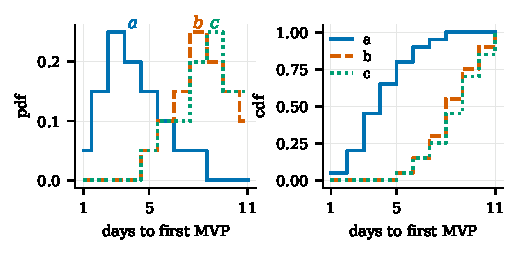
\includegraphics[width=.9\linewidth]{fig/stats_xdf}
\caption{Twenty runs per framework: days to first MVP, as
probability density functions (left) and cumulative
distribution functions (right).
Frameworks $b$ and $c$ overlap almost everywhere; $a$ is
several days faster.
Regenerate with \texttt{make statsfig}.}
\label{fig:xdf}
\end{figure}

\subsection{Two Questions, One Verdict}

Statistical comparisons answer two different questions.
A significance test asks: could a gap this large be chance?
An effect size asks: is the gap big enough to matter?
The two can disagree: given enough runs, even a microscopic
difference passes a significance test, while with too few runs,
even a large difference can be luck.
One check guards against noise, the other against triviality;
hence standard advice runs both~\cite{arcuri11}.

Our code adds one more safeguard.
Effect sizes come in parametric and non-parametric flavors, and
each can be fooled in its own way, so both flavors are run.
Two samples are called ``the same'' only when all three tests
agree that the difference is small: two effect sizes
(\texttt{cohen}, \texttt{cliffs}) and one significance test
(\texttt{ks}), each defined in the sections that follow.
Python's \texttt{and} is lazy, so the cheapest test runs first
and the costlier ones run only when needed.

Every test here expects sorted input; that one convention buys
linear scans, percentile tricks, and free medians throughout.
By default \texttt{same} trusts its caller to pre-sort (as
\texttt{ranks} does below); pass \texttt{is\_sorted=False}
and it sorts defensively first.

\begin{lstlisting}[style=py]
def same(xs, ys,
         c0=.35,   # cohen threshold; from |\cite{cohen88,sawilowsky09}|
         d0=.195,  # cliffs threshold; from |\cite{romano06}|
         k0=1.36,  # ks threshold; from |\cite{massey51}|
         is_sorted=True):
    if not is_sorted:
        xs, ys = sorted(xs), sorted(ys)
    return (cohen(xs, ys)  <= c0 and
            cliffs(xs, ys) <= d0 and
            ks(xs, ys)     <= k0)
\end{lstlisting}

On the worked example of \S\ref{sec:worked}, all three tests
agree:
\begin{itemize}
	\item
Comparing $b$ to $c$ yields $d\!=\!0.13$, $\delta\!=\!0.10$,
and $\mathit{ks}\!=\!0.32$: all under their thresholds, so
\texttt{same} returns true.
\item
Comparing $a$ to $b$ yields $d\!=\!2.2$, $\delta\!=\!0.91$, and
$\mathit{ks}\!=\!2.4$: all far over, so \texttt{same} returns
false.
\end{itemize}
Taken together, those verdicts divide the three frameworks into
two groups:
\begin{center}
\texttt{( (a), (b, c) )}
\end{center}
The eyeball intuition is now a defensible claim.

For code that reports these groupings, see 
\S\ref{sec:ranks}.

\subsection{Significance: the Kolmogorov--Smirnov Test}

\textbf{Means} can agree while distributions disagree; e.g.
two samples can share an average while one is tight and the
other is spread wide.
The Kolmogorov--Smirnov statistic guards against this by
comparing whole cumulative distributions~\cite{massey51}.
The intuition runs as follows.
If two samples come from the same source, their cdfs should
ride on top of each other: at every value, about the same
fraction of each sample lies below.
Anywhere the curves pull far apart, one treatment has finished
far more of its runs than the other, so the distributions must
differ.

The KS statistic reports the  largest vertical gap between cdfs.
For example,
Figure~\ref{fig:ks} repeats the cdfs of
Figure~\ref{fig:xdf}, now with that gap drawn in
(so the KS
statistic is the tallest pole that fits between two cdfs).
Between $a$ and $b$ the pole is tall ($D\!=\!0.75$); between
$b$ and $c$ no pole higher than $D\!=\!0.10$ fits anywhere.

\begin{figure}[t]
\centering
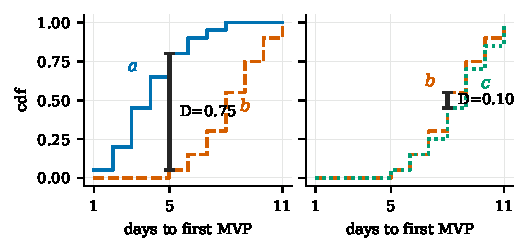
\includegraphics[width=.9\linewidth]{fig/stats_ks}
\caption{The KS statistic is the largest vertical gap between
two cdfs (the black pole).
Left: $a$ versus $b$.
Right: $b$ versus $c$.
Regenerate with \texttt{make statsfig}.}
\label{fig:ks}
\end{figure}
The code walks both sorted lists one distinct value at a time,
advancing two counters \texttt{p} and \texttt{q} past ties, so
the whole pass is linear.
After each advance, \texttt{p/nx} and \texttt{q/ny} are the two
cdfs sampled at the same value \texttt{v}.
Dividing the raw gap by $\sqrt{(n_x+n_y)/(n_x n_y)}$ rescales
it into critical units; at the usual five-percent false-alarm
rate, the \textbf{critical value} on that scale is the tabled
constant $1.36$~\cite{massey51}, so results under $1.36$ are
insignificant.

\begin{lstlisting}[style=py]
def ks(xs, ys):
    nx, ny = len(xs), len(ys)
    d = p = q = 0
    while p < nx and q < ny:
        v = min(xs[p], ys[q])
        while p < nx and xs[p] == v: p += 1
        while q < ny and ys[q] == v: q += 1
        d = max(d, abs(p/nx - q/ny))
    return d / ((nx + ny) / (nx * ny)) ** 0.5
\end{lstlisting}

\subsection{Effect Size}

Two effect sizes are used here: one non-parametric
(Cliff's $\delta$) and one parametric (Cohen's $d$).

\subsubsection{Rank Imbalance: Cliff's $\delta$}

Cliff's $\delta$ is a non-parametric effect
size~\cite{cliff93}.
It asks: if one item is drawn from each sample, how often does
$x$ beat $y$, minus how often $y$ beats $x$?
Naively that is a quadratic all-pairs count.
Sorting first makes it linear: as \texttt{x} ascends, the
counts \texttt{j} and \texttt{k} (how many \texttt{ys} sit
below, and at-or-below, \texttt{x}) only ever move forward.
Romano et al.\ rate $\delta<0.147$ as negligible and
$\delta<0.33$ as small~\cite{romano06}; our threshold of
$0.195$ splits that range, a slightly strict ``smallish.''

\begin{lstlisting}[style=py]
def cliffs(xs, ys):
    gt = lt = j = k = 0
    for x in xs:
        while j < len(ys) and ys[j] < x: j += 1; k = j
        while k < len(ys) and ys[k] == x: k += 1
        gt += j; lt += len(ys) - k
    return abs(gt - lt) / (len(xs) * len(ys))
\end{lstlisting}

\subsubsection{Pragmatic Dullness: Cohen's $d$}

Sooner or later, a business user reviewing statistical results
will say: ``that difference may be real, but it is dull; I only
care about deltas bigger than $x$.''
The complaint bites hardest when results are printed rounded: a
difference can pass both tests above, yet be smaller than the
last digit shown.
Hence one more test is needed, one that can call a difference
real but pragmatically insignificant.
Cohen's $d$ is the standard test for dull: the gap between two
means, in units of the pooled \textbf{standard
deviation}~\cite{cohen88}.
Cohen rated $d\!=\!0.2$ as small and $d\!=\!0.5$ as
medium~\cite{cohen88} (Sawilowsky later refined that
scale~\cite{sawilowsky09}); our threshold of $0.35$ is the
border between the two, so gaps under about a third of a
standard deviation count as dull.
If no such pragmatic argument is needed, set \texttt{c0} to
infinity in \texttt{same} and \texttt{cohen} loses its vote.

The pooled deviation weights each sample's \textbf{variance} by
its degrees of freedom, so unequal sample sizes are handled
fairly.
A \texttt{TINY} constant guards the division when both samples
have near-zero spread.
The code needs no imports: on sorted data, the gap between the
10th and 90th percentile spans 2.56 standard deviations of a
normal curve, so one subtraction estimates the deviation.

\begin{lstlisting}[style=py]
TINY = 1e-32

def mean(a): return sum(a) / len(a)
def stdev(a): n = len(a)//10; return (a[9*n]-a[n])/2.56

def cohen(xs, ys):
    n, m = len(xs), len(ys)
    sd = (((n-1)*stdev(xs)**2 +
           (m-1)*stdev(ys)**2) / (n+m-2)) ** 0.5
    return abs(mean(xs) - mean(ys)) / (sd + TINY)
\end{lstlisting}

\subsection{Ranking Many Treatments}
\label{sec:ranks}

Real studies compare many treatments, not two.
Running all pairwise tests invites false alarms, so instead the
treatments are sorted by their \textbf{medians}, then swept
once from best to worst.
Each treatment is compared to the best member of the current
\textbf{rank}; when \texttt{same} says they are indistinguishable, the
rank is shared, otherwise a new rank opens.
Rank zero holds the winners; the full table maps every
treatment to its rank.
The flag \texttt{big} flips the sort for measures where larger
is better.

\begin{lstlisting}[style=py]
def ranks(d, big=False):
    mid  = lambda t: t[len(t) // 2]
    dd   = {k: sorted(v) for k, v in d.items()}
    out, win, rank, best = {}, [], -1, None
    for k in sorted(dd, key=lambda k: mid(dd[k]), reverse=big):
        if best is None or not same(dd[best], dd[k]):
            rank, best = rank + 1, k
        if rank == 0: win.append(k)
        out[k] = rank
    return win, out
\end{lstlisting}

Applied to the worked example (where fewer days is better, so
\texttt{big} stays false), \texttt{ranks} sorts the frameworks
by their medians (4, 8, 9 days), gives $a$ rank zero, then
finds $b$ and $c$ indistinguishable, so they share rank one.
That is, this data forms two groups:
\begin{center}
\texttt{( (a)~~(b c) )}
\end{center}
and the winners list is just $[a]$.

Note the single sort at the top of \texttt{ranks}: every later
test then runs on pre-sorted lists, so the whole ranking costs
one sort per treatment plus one linear sweep.

Results sections often end with a chart like
Table~\ref{tbl:grid}: here, ten treatments are compared on ten
data sets, twenty runs per cell.
Grey marks the top-ranked treatments of each data set; the
bottom row counts how often each treatment reaches the top
rank.
Such a chart supports a one-sentence summary: rx7 wins over
everything else (but see db2 and db5 for counterexamples).
The result is a statistics stack small enough to audit in an
afternoon, yet defensible enough for a results section.

\begin{table}[!t]
\caption{Ten treatments (rx1..rx10) on ten data sets
(db1..db10).
Cells show the median of twenty runs (fewer is better); grey
cells sit at the top rank of their data set, as computed by
\texttt{ranks}; the bottom row counts top-rank appearances.
Summary: rx7 wins over everything else, but see db2 and db5 for
counterexamples.
Regenerate with \texttt{make statsfig}.}
\label{tbl:grid}
\centering\small
\setlength{\tabcolsep}{2.5pt}
\begin{tabular}{@{}l*{10}{r}@{}}
\toprule
 & rx1 & rx2 & rx3 & rx4 & rx5 & rx6 & rx7 & rx8 & rx9 & rx10\\
\midrule
db1 & 8.2 & 9.7 & 11.1 & 12.0 & 14.5 & 8.0 & \cellcolor{black!15}5.3 & 10.9 & 12.7 & 14.1\\
db2 & 8.4 & \cellcolor{black!15}3.1 & 11.0 & 11.9 & 14.3 & 8.5 & 12.4 & 11.3 & 12.5 & 14.1\\
db3 & 8.7 & 9.7 & 10.9 & 12.4 & 13.8 & 7.9 & \cellcolor{black!15}5.5 & 11.3 & 12.5 & 13.9\\
db4 & 8.2 & 9.6 & 11.0 & 12.7 & 14.0 & 8.0 & \cellcolor{black!15}5.4 & 11.1 & 12.6 & 14.2\\
db5 & 8.3 & 9.2 & 11.3 & 12.7 & \cellcolor{black!15}3.2 & 8.1 & 12.5 & 11.2 & 12.5 & 14.0\\
db6 & 8.1 & 9.7 & 10.9 & 12.5 & 14.2 & 8.4 & \cellcolor{black!15}5.1 & 10.9 & 12.1 & 14.3\\
db7 & 8.2 & 9.7 & 11.2 & 12.7 & 14.3 & 8.3 & \cellcolor{black!15}5.2 & 10.5 & 12.7 & 14.4\\
db8 & 8.4 & 9.5 & 11.3 & 12.7 & 13.7 & 7.8 & \cellcolor{black!15}4.7 & 10.6 & 12.2 & 14.1\\
db9 & 8.1 & 9.5 & 10.7 & 12.5 & 13.7 & 8.2 & \cellcolor{black!15}5.1 & 11.2 & 12.5 & 14.0\\
db10 & 8.5 & 10.0 & 11.1 & 12.5 & 13.9 & 8.5 & \cellcolor{black!15}5.2 & 10.9 & 12.9 & 14.0\\
\midrule
wins & 0 & 1 & 0 & 0 & 1 & 0 & 8 & 0 & 0 & 0\\
\bottomrule
\end{tabular}

\end{table}


\end{document}
